\chapter{Approaches for analyzing and predicting Customer Satisfaction}
\label{ch:implementation}

This chapter of the thesis focuses on the design and implementation of promising approaches which were introduced and described in more detail within the previous chapter. 

\section{Identification of relevant data sources}
\label{sec:dataSources}

On the one hand, statistical analysis and data-driven approaches are rich tools to gain new insights into the data and find hidden associations and relationships but on the other hand these approaches will not deliver any satisfying results if they work with wrong or invalid datasets as input. Therefore it is essential to invest enough resources on selecting relevant data sources and ensuring high quality within this data before starting with any analytical approach. Considering right and valid data was not only mentioned once in literature as a key factor for successful data analysis \cite{neckel2015}. 

\subsection{Selecting the right data based on its representativeness regarding Customer Satisfaction}

The approach this thesis followed for selecting relevant data sources is based on the definition of Customer Satisfaction as it was modeled in section~\ref{ssec:customerSatisfaction}. Furthermore, as already indicated in section~\ref{ssec:customerSatisfaction}, the focus is on the provided service quality and customer usage, since these metrics can be represented in data and as a result are measurable. First of all, the proceeding started with a summarization of properties and features of the main product considered in the use case scenario, namely the Tractive GPS device, are advertised actively to potential customers. As representative resource the landing web page of the company, namely https://www.tractive.com, was used to extract this information. This website is the major source of customer conversion  and lists all relevant characteristics and features of the product. Figure \ref{fig:tractiveLanding} shows an extract of this web page.

\begin{figure}
	\centering
	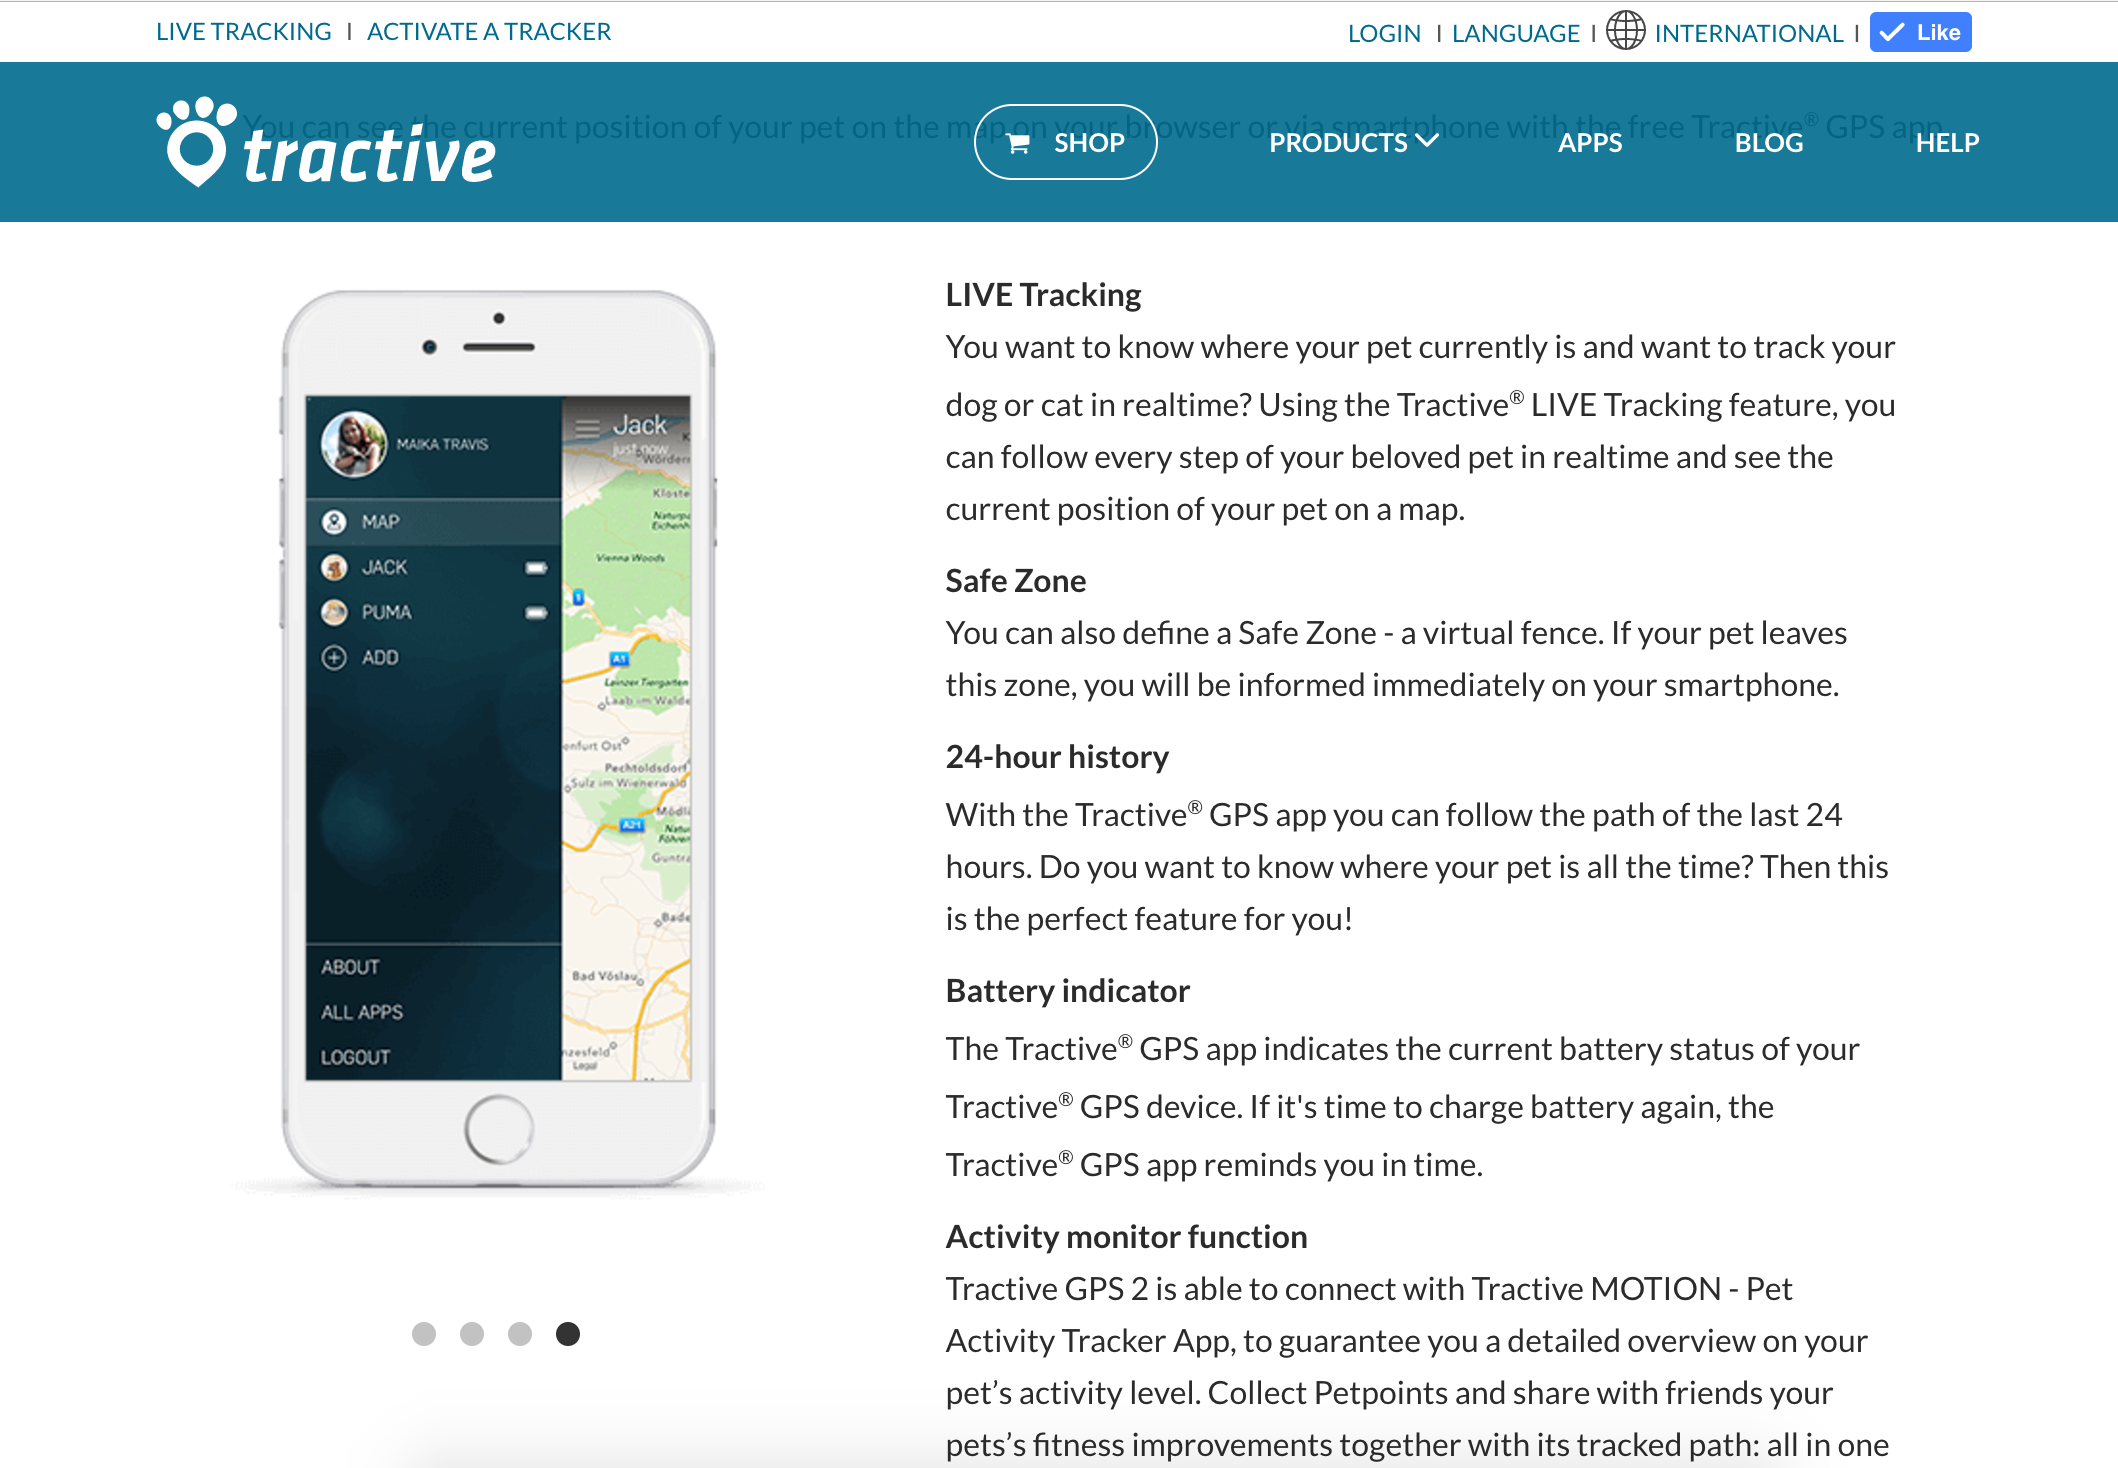
\includegraphics[width=1.0\textwidth]{img/tractiveLanding.png}
	\caption{Extract of landing page https://tractive.com}
	\label{fig:tractiveLanding}
\end{figure} 

Other sources used in marketing like social media channels provide brief summarizations of this content and link to the main website. Therefore it can be implied that product descriptions on the landing web page are decisive for customers and drive their expectations with regard to the product. Table~\ref{tab:productFeatures} gives an overview on important properties and features regarding Tractive GPS from a customer's perspective. Moreover, it assigns the data which will be useful for reasoning about Customer Satisfaction. It indicates what a customer can expect when he purchases the product.

\begin{table}[]
	\centering
	\resizebox{\textwidth}{!}{%
		\begin{tabular}{|l|l|l|}
			\hline
			\multicolumn{1}{|c|}{\textbf{Feature / Characteristic}} & \multicolumn{1}{c|}{\textbf{Description}} & \multicolumn{1}{c|}{\textbf{\begin{tabular}[c]{@{}c@{}}Nature of data suitable for \\ predicting Customer Satisfaction\end{tabular}}} \\ \hline
			Locate pet anytime, anywhere & \begin{tabular}[c]{@{}l@{}}See location of pet accurately \\ on a map on the Smartphone\end{tabular} & Position data (GPS, Mobile Cell) \\ \hline
			Live Tracking & \begin{tabular}[c]{@{}l@{}}Follow the trace of a pet in \\ realtime on a smartphone\\ or on a web page\end{tabular} & Live Tracking commands statistics \\ \hline
			Safezones & \begin{tabular}[c]{@{}l@{}}Creating a virtual fence and \\ get notified if pet leaves \\ selected safe area\end{tabular} & \begin{tabular}[c]{@{}l@{}}Number of times pet leaves \\ and enters safezone,  \\ reliability data regarding notifications\end{tabular} \\ \hline
			Battery indication & \begin{tabular}[c]{@{}l@{}}If battery of GPS device is \\ full or is nearly empty, \\ it will be indicated \\ in the Smartphone app\end{tabular} & \begin{tabular}[c]{@{}l@{}}Reliability of data regarding \\ battery notifications\end{tabular} \\ \hline
			Integrated light & \begin{tabular}[c]{@{}l@{}}Customers can turn on the \\ integrated LED (Light-Emitting Diode) \\ on the GPS device \\ via the Smartphone\end{tabular} & LED command statistics \\ \hline
			100\% waterproof & \begin{tabular}[c]{@{}l@{}}A product characteristic \\ customers trust in, since many \\ pets often get wet\end{tabular} & \begin{tabular}[c]{@{}l@{}}Hardware defects due to \\ water damage\end{tabular} \\ \hline
			Premium Customer Service & \begin{tabular}[c]{@{}l@{}}With a premium service plan, \\ it is promised that customers \\ get feedback within 24 hours \\ on weekdays\end{tabular} & \begin{tabular}[c]{@{}l@{}}Customer service data related \\ to ticket resolving times\end{tabular} \\ \hline
		\end{tabular}%
	}
\caption{Features / characteristics of product among with their nature of data suitable for predicting Customer Satisfaction.}
\label{tab:productFeatures}
\end{table}

The table excludes properties which are advertised but where the nature of the feature is static and stays always the same among all customers. Such properties are usually product characteristics which do not change due to customer use and as a result are not measurable in collected data. An example is the handy charging unit or the fact that the GPS device is one of the smallest and lightest devices for pet tracking available on the market. From a marketing point of view these are essential characteristics but with regard to this thesis they are neglectable due to the reason that they ar independent of customer usage behavior. 

\subsection{Elaboration on data collection regarding identified features}
This section will have a detailed look into availability, representation and content of stored data for the features from table~\ref{tab:productFeatures}. The procedure this thesis followed for this task started with an investigation to find out by which of the data collections each feature is represented best and how much value in the content is included. Following paragraphs assign identified data sources to categories and introduce a structure which makes it more understandable for the reader. It is not the aim of the following paragraphs to discuss every data attribute which could contribute to predicting Customer Satisfaction in depth. Instead the following paragraphs will rather explain briefly which type of data is stored in the collections and how the data is generated due to a customers behavior. The idea is to get a sense for why they would be important when it comes to Customer Satisfaction prediction.

\subsubsection{Device related data}
\label{sssec:deviceRelatedData}
This group contains a bunch of potentially valuable data resulting from device usage. This type of data is created by sending of data from the device to a backend service and storing it in the database or sending commands from a client to the backend and finally to the device which should initiate some action. Before looking on concrete schemata of the data, figure~\ref{fig:tractiveDataFlow} illustrates in a simplified way the communication and thus the data exchange between client and device. 

\begin{figure}
	\centering
		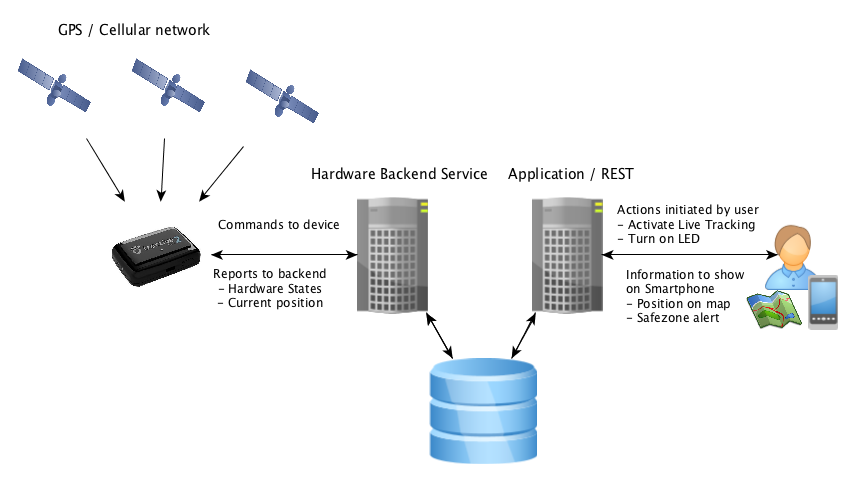
\includegraphics[width=1.0\textwidth]{img/tractiveDataFlow.png}
	\caption{Overview on communication and data flow between client and device}
	\label{fig:tractiveDataFlow}
\end{figure}

The following list outlines the essential device related data collections leveraged in the analytical part of the thesis. 

\begin{itemize}
	% TODO: Find out how often is it actually sent when the tracker is on
	\item \textbf{Device id reports} are sent automatically from time to time when the tracker is switched on and has network coverage. The Id reports contain information about the firmware- and hardware version of the device. Since there are bug fixes and improvements on the firmware quite often and updating it on a device is possible over the air, this can lead to differences in service quality among devices. Furthermore the device id reports allow to imply the activity level (eg.: the number of days in use) of a customer's tracker.
	\item \textbf{Device position reports}: Every time a tracker receives a position it is stored in the database. Along with the latitude and longitude of the position there is data indicating whether GPS or mobile cell network was used for localization, how strong the received signal was, as how accurate the position is classified, the timestamp when the device received the position, the time where it was stored in the database and some further technical GPS data as the number of reachable satellites used for localization. 
	\item \textbf{Device network reports} contain data about current network coverage. Since the device can be used in over 100 countries worldwide each network report provides the MCC (Mobile Country Code) which indicates where the device is currently used. Prior experiences showed that network coverage sometimes varies a lot among countries which can influence satisfaction of a customer. The mobile network generation which is limited to GSM and UMTS in the use data of this thesis can have an impact as well.
	\item \textbf{Device hardware reports}: These reports are usually sent along with the id reports described before and contain different kind of hardware states. Interesting attributes are for instance the current battery level- and voltage, temperature states or collected number of position, error and network logs for the particular device. Moreover hardware reports store specific hardware events for a point in time where they happened. Amongst others this includes valuable information as the time when the device has been switched on/off or battery is charging, full or low. 
	\item \textbf{Geofence reports}: If a customer's pet with a mounted device leaves or enters a virtual fence defined in the app, a geofence report with trigger (called In-break in case of entering the safezone or Out-break otherwise) and source (GPS or mobile cell) is sent to the server which stores it into the database and initiates sending a push or mail notification to the customer. Both accuracy based on the trigger source and the number of In- and Out-breaks can influence Customer Satisfaction. 
	\item \textbf{Server commands}: These are commands which are sent due to an action initiated by the user. The most prominent server command according to the statistics so far is the Live Tracking function where the device starts sending a new position every few seconds for a maximum of ten minutes which allows the user to follow his/her pet in real time. Further commands enable the user to turn on/off the integrated light or trigger a sound on the device. The server commands are very essential for customers of the Tractive GPS device and therefore several attributes indicating the quality are collected. For each server command the timestamps when the command was sent by the server to the device, when it was commanded by the device and the time of confirmation respectively cancellation by the device is recorded. 
\end{itemize}

\subsubsection{Notification related data} 
% TODO: Check again if really every notification attempt is stored in push logs %
Notifications play an essential role for Tractive customers, since the information whether a pet has left a defined safezone or the battery state of the device is critical can be crucial for users. The assumption made in this thesis relies on the fact that reliability of notification delivery either via mail but even more important via push on the Smartphone has an influence on Customer Satisfaction. As mentioned in the device related data geofence reports are sent in case the device is not within the safezone area and stored in the database. Any mail- and push notification sending attempts no matter whether they were successful or not are stored in push logs. Each push log entry contains a reason for sending it, the message, a reference to the tracker in case of a safezone- or battery alert and the return status indicating the success state. 

\subsubsection{Customer service related data}
Tractive advertises a first-class customer service which a lot of customers actually make use of. Tractive for instance promises feedback within 24 hours. Instead of responding to formless emails, Tractive employs the popular customer support service tool Zendesk® which is the central place for desires, complaints and support requests. Next to better data integration there is the advantage that all collected information regarding a particular support ticket is stored transparently and can be retrieved if needed. Thus, this enabled the opportunity to analyze the time passed until a ticket is handled which is also assumed to have an impact on the overall satisfaction of customers.

\subsection{Quality of identified data and preprocessing}
The relevant data sources are identified but before diving into the implementation of analytical processing the thesis took a look into quality of the data and modified or enriched it if considered as necessary. The aim was to provide correct and analytical oriented data as input for the actual analysis and data-driven approach. 

\subsubsection{Representation in database system}
As \cite{neckel2015} outline in their research, one of the major prerequisites for a successful data analysis is that the available data provides a unique view on the real world and prevents ambiguous data collections. Tractive uses the semi-structured NoSql database MongoDB as central storage system for any transactional customer and device related data. This has the big advantage that identified data sources can be taken from the same database system and thus provide a unique interface to query sample data for analysis and prediction. Since this thesis considers data generated by customers using a Tractive GPS device, inconsistencies among transactional-driven data are not a problem as it often is the case for companies with a diverse product palette \cite{neckel2015}.

\subsubsection{Transactional- vs. analytical oriented data}
When taking a look on the nature of the selected data, it can be noticed that it results from operative application. Although this huge amount of transactional data provides the opportunity for intensive analyses, it is not always on the desired level of detail. This was realized during the first few analysis steps and made it necessary to bring some data collections in another format. Section ~\ref{sssec:deviceRelatedData} outlined the server commands as critical contributor to Customer Satisfaction. However, the collected data attributes belong to one particular server command of a device. This would require extra calculations for each device during analysis to aggregate command success rates or delays. Moreover other device related information like the model edition, batch number, country of use or SIM provider is stored in another collection and therefore not directly available. 

% TODO: Check if it really was mid of may %
Due to the importance of these server commands for its business, Tractive decided to store beginning with mid of May the server commands in addition in a suitable form to make analysis, statistical evaluation and trend analysis more convenient. Therefore a new collection, namely server command metrics, was created. From this point in time on, every new server command causes a new entry in the metrics collection with a reference to the user who initiate the action, to the device along with its properties to filter and the server command specific information delivered from the hardware device itself. An extract of the schema of this collection is shown in table~\ref{tab:serverCommandMetrics}. 

\begin{table}[]
	\centering
	\resizebox{\textwidth}{!}{%
		\begin{tabular}{|l|l|}
			\hline
			\multicolumn{1}{|c|}{\textbf{Attribute names}} & \multicolumn{1}{c|}{\textbf{Description}}                                                               \\ \hline
			hw\_edition                                    & \begin{tabular}[c]{@{}l@{}}One of the three available\\ editions. (Normal, Pink or Hunter)\end{tabular} \\ \hline
			batch\_no                                      & Batch number                                                                                            \\ \hline
			sim\_type                                      & SIM provider                                                                                            \\ \hline
			iso2                                           & Country code of usage                                                                                   \\ \hline
			cmd\_success\_rate                             & \begin{tabular}[c]{@{}l@{}}Percentage of successfully\\ issued commands\end{tabular}                    \\ \hline
			cmd\_cancelled\_rate                           & Percentage of canceled commands                                                                         \\ \hline
			cmd\_terminated\_rate                          & Percentage of terminated commands                                                                       \\ \hline
			cmd\_delay\_to\_commanded                      & \begin{tabular}[c]{@{}l@{}}Delay until command is \\ received at device\end{tabular}                    \\ \hline
			cmd\_delay\_to\_confirmed                      & \begin{tabular}[c]{@{}l@{}}Delay until command is successfully\\ confirmed by the device\end{tabular}   \\ \hline
			cmd\_delay\_to\_pos\_any                       & \begin{tabular}[c]{@{}l@{}}Delay until any position is \\ available\end{tabular}                        \\ \hline
			cmd\_delay\_to\_pos\_new                       & \begin{tabular}[c]{@{}l@{}}Delay until a new position \\ is available\end{tabular}                      \\ \hline
			cmd\_duration                                  & Whole duration of a command                                                                             \\ \hline
		\end{tabular}%
	}
	\caption{Important attributes of aggregated server command metrics to be used for data analysis}
	\label{tab:serverCommandMetrics}
\end{table}

After one month of storing those metric entries for each device when a new server command is executed, it was decided to make use of this data within the thesis instead of relying on the transactional entries. The main advantage using this preprocessed analytical oriented data will be revealed when diving deeper into the querying tasks during data analysis. 

Alongside with prominent advertised features, the work in this data gathering and preprocessing task also took opinions, complaints or desires under consideration to get a feeling of what additional properties seem to be useful for customers and make them (un)happy. Due to the lack of automatism, feedback from Tractives customer support service employees was considered as source of trust. It turned out that the battery life of a device, which is not advertised explicitly on the landing web page of Tractive, was often mentioned in contact with customers. As a result of these findings, the author of this thesis decided to include battery life time of devices in the Customer Satisfaction prediction approaches. 

Due to the reason that battery levels are only reported as single events within hardware reports it was necessary to compute battery life time with following approach. % TODO: Describe calculation of battery life time if it will be used within practical work

\section{Hypotheses-driven approach to gain knowledge about interrelationships among data}

% TODO: Change first reference to final section in second chapter introducing analysis approaches
Based on the prepared data analysis work started with a top-down approach as it was described in section~\ref{ch:backgroundResearch}. The aim was to get an understanding which types of data influence the output of other data and how strong these correlations are. In essence, the overall goal was to reveal which of the data related to customer usage is expressive regarding Customer Satisfaction. For this type of analysis, hypotheses were explicitly defined and either verified or falsified by statistical measurements. It was planned to use results if they are promising for a manual feature selection in an automatic framework for Customer Satisfaction prediction. 

\subsection{Choosing target data approximating Customer Satisfaction}

While section~\ref{sec:dataSources} explored the available data sources to identify those which are likely to be predictors for Customer Satisfaction, the work explained in this section tried to find data reasoning about an effect on Customer Satisfaction. This target data should be as expressive to distinguish satisfied and dissatisfied customers. Due to the lack of any explicit satisfaction responses, implicit data instead had to be found. The author of this thesis proceeded by finding behavioral patterns customers would follow if they feel pleased or disappointed and came up with following collected data:

\begin{itemize}
	\item Recurring service active or canceled: The assumption hereby is that on the one hand satisfied customers will keep their service where they pay monthly, yearly or biennially active and are therefore able to use the device anytime. On the other hand dissatisfied customers are vulnerable to cancel the service and leave the relationship with the company. These thoughts are based on the theory of relationship between Customer Satisfaction and loyalty outlined in sections~\ref{ssec:customerSatisfaction} and~\ref{ssec:custLoyalty}.
	\item Increased or diminished app usage: The assumed behavioral property resulting from (dis)satisfaction is that customers increase respectively diminish the usage of the smartphone app. According to the analytics data the Tractive GPS app for iOS and Android is most important for customers of a Tractive GPS device. As a result of good user experience it is expected that customers use the app more often and the same vice versa. The data indicating events for opening the app on a smartphone as well as bringing the app into foreground were taken as representative indicators.
	\item How many days GPS device is in use: The device id reports also mentioned in section~\ref{sssec:deviceRelatedData} can be seen as an activity indicator when aggregated over a period of time. The thesis considered the number of days the device sent id reports as a meaningful number depending on increased of decreased satisfaction.
\end{itemize}

\subsection{Formulation of Hypotheses and solving analysis problem}
Before setting up the specific hypotheses and choosing the statistical tools to prove them, a so called CRM problem was defined for this top-down approach. From a business point of view it is important to find out key factors driving satisfaction of customers to put more effort in improving them and in the end increase company value by binding customers permanently. For an automatic customer satisfaction prediction those key factors should help for selecting the right features more easily. The procedure followed has been described in section~\ref{ch:backgroundResearch}. The upcoming paragraphs give a more detailed insight into the different hypotheses tested, how they were checked and which statistical tools were applied. The analysis task can be split into two types of data, namely categorical- and continuous data.

\subsubsection{Analysis of categorical data}
This first analysis done in the implementation part of this thesis is based on the relationship between customer- satisfaction and loyalty. Thus it took a look on the long-term relationship of a customer with Tractive. Only the service status "Active" which indicates that a customer is paying on a recurring basis and the service status "Terminated" which indicates a manual service cancellation by a customer were considered. This implies the fact, that this task relies on binary categorical data. The analysis goal was then stated as: Does Live Tracking success influence service termination behavior? 

\begin{enumerate}
	\item Hypotheses
	\begin{description}
		\item[H0] There is no significant difference in service termination behavior between customers who belong to the group of bad live-tracking users and customers who belong to the group of good live-tracking users.
		\item[H1] There is a significant difference between these two groups.
	\end{description}
	\item Analysis objects
	\begin{itemize}
		\item Live Tracking Server commands related to a specific tracker
		\item Service status of customers
	\end{itemize}
	\item Analysis problem
	\begin{itemize}
		\item Select representative sample and split it up into two groups to compare, namely a treatment and control group.  It is important to exclude any other influencing factors as best as possible and therefore define common base data shared among both groups. 
		\item Choose a suitable sample size
	\end{itemize}
	\item Analysis solution: Statistical test which should check whether the Null-hypothesis can be rejected and thus statistical significant difference can be shown. The analysis was done on 17.04.2017. 
	\begin{itemize}
		\item Group selection: The first group contains random customers suffering from bad Live Tracking which was defined by an overall success rate below 70\%. In contrast, the control group consists of customers with a success rate greater or equal than 80\%. These thresholds were set according to experience in customer support where complaints from users regarding Live Tracking usually show success rates around this threshold. As common base data only users from Germany who own at least one Tractive GPS device and do not have a premium service plan to be payed on a monthly basis which was created before 01.10.2016 and is at least valid until 01.10.2016 were considered. 
		\item Choose a suitable sample size: The sample size for the two groups was estimated based on findings of \cite{campbell1995estimating}. Regarding statistical significance a widely used $\alpha$-error of 5\% was used while a $\beta$-error of 10\% should clearly reduce the probability of false-negatives meaning non-rejection of H0 although it could have been rejected. Since a statistical significant result does not necessarily say something about expressiveness of the computed result, a minimal relevance level had to be set for choosing an appropriate sample size. A 20\% decrease of active subscriptions due to bad Live Tracking was considered as relevant. Picking the right number from the proposed sample size table yielded a number of 79 per group which in total is 158. 
		\item Querying data: At the time where this particular analysis was conducted no analytical view on the server command metrics was available and therefore the procedure was to calculate those metrics for the devices under consideration on the fly. Therefore a Javascript program was implemented to fetch randomly the necessary number of subscriptions which either had status "active" or "terminated" with the defined common data. Based on the device reference, server commands of type "Live Tracking" within the given time period were filtered and the success rate averaged. Based on the output data a post-processing step provided a simple 2x2 table which is illustrated in~\ref{tab:binaryLtData}. 
		
		\begin{table}[]
			\centering
			\resizebox{\textwidth}{!}{%
				\begin{tabular}{|l|l|l|}
					\hline
					\multicolumn{1}{|c|}{\textbf{}} & \multicolumn{1}{c|}{\textbf{Service status = ACTIVE}} & \textbf{Service status = TERMINATED} \\ \hline
					\textbf{Good Live Tracking}     & 54                                                    & 8                                    \\ \hline
					\textbf{Bad Live Tracking}      & 43                                                    & 19                                   \\ \hline
				\end{tabular}%
			}
			\caption{2x2 table showing influence of Live Tracking on service status}
			\label{tab:binaryLtData}
		\end{table}
		\item Use statistical test to verify or falsify H0: There are different statistical tests for binary data whereby Fisher's exact test is proposed as most suitable for a rather small sample size as it was in this case \cite{raymond1995exact}. The test works based on a 2x2 table as input and calculates a 95\% confidence interval indicating where the true odd ratio lies. The odds ratio is a often used value when analyzing binary data and states the relative probability than an event occurs against that it does not occur \cite{bland2000odds}. The Null-hypothesis in Fisher's exact test can be rejected if the confidence interval does not include the odds-ratio 1. Then it is safe to claim that there is a difference between the two sample groups under consideration. The open source statistic program package R was used to execute the Fisher exact test for the 2x2 table and yielded a confidence interval of $[1.105933, 8.604534]$ which indeed allows rejecting H0. Based on this statistical experiment it is thus valid to say that there is a statistical significant and based on the minimum of 20\% difference in terminations between treatment and control group also a relevant result.
		\item Interpreting the result: This data analysis confirms the expected importance of the Live Tracking function for Tractive's customers since terminating an active service is equal to ending the relationship with the company and can therefore be considered as a last resort in case of dissatisfaction. As a result it can be stated that Live Tracking success rate qualifies as potentially promising feature for Customer Satisfaction. 
	\end{itemize}
\end{enumerate}

\subsubsection{Analysis of continuous numeric data}
The following analysis tasks are all based on continuous data and therefore summarized in this section. Although the procedure remained the same as explained in the previous section, all sub-tasks share some common ground and therefore it was decided to make the analysis more modular. As a result of this decision, a NodeJS application with a MongoDB connection driver was created. Querying tasks were extracted into reusable Javascript functions. Before elaborating on the particular sub-tasks, the common parts are described following:

\begin{itemize}
	\item Choose a suitable sample size: For an appropriate choice the width of the confidence interval, where the true correlation coefficient of the population lies, was considered. The author decided on 0.1 as its width for the experiments to ensure a high precision. Since the app usage was not considered as a direct measurement of a customer satisfaction value, a sample correlation coefficient of 0.4 was determined as relevant. Based on these parameters and the research of \cite{moinester2014sample} a sample size of 1086 could be derived for the correlation analyses. 
	\item Select sample users: The selection was done by randomly skipping users and ended when the maximum sample size of 1086 was reached. For every sub-task only users with exactly one active service were considered to make comparison with device related data easier. The output of this selection stage contained user- and device ids.
	\item Query data to compare: Data from the previous stage was used as input parameter for the according function to fetch the desired data rows for correlation analysis within a selected time period. The implemented queries heavily use the aggregation framework of MongoDB to provide the desired data in an aggregated form grouped by user id. 
	\item Match data based on user id: The data collected was stored in JSON (Javascript Object Notation) arrays in-memory. A matching function finally generates the input vectors for the subsequent statistical calculations, by matching the nested JSON objects via the user id and writing data to one CSV file each. 
	\item Use correlation analysis to reason about linear relationship: After finishing the querying part, the data was ready for correlation analysis. Therefore the statistical open source program package R was used to calculate a Bravai-Pearson correlation coefficient and thus get a first impression on the relationship between the considered data rows.  
\end{itemize}

Following correlation analyses were done with the aim to find influencing factors for Customer Satisfaction.
The ordered list below shows the analysis goal implicitly formulating the hypotheses along with the data collections used for each analysis and the results retrieved.

\begin{enumerate}
	\item Do server command metrics cause an increased respectively diminished app usage?
	\begin{enumerate}
		\item Analysis objects
		\begin{itemize}
			\item Server command metrics collection
			\item App Events collection containing app startup and app foreground events
		\end{itemize}
		\item Results: See table~\ref{tab:serverCommandsAppUsage}
		\begin{table}[]
			\centering
			\resizebox{\textwidth}{!}{%
				\begin{tabular}{|l|l|l|l|}
					\hline
					\textbf{Date of analysis} & \multicolumn{1}{c|}{\textbf{Commands}} & \multicolumn{1}{c|}{\textbf{Attribute}} & \textbf{Correlation coefficient} \\ \hline
					04.06.2017                & LT                                     & Command success rate                    & r = 0.04222696                   \\ \hline
					04.06.2017                & LT, Buzzer, LED, Position request      & Command success rate                    & r = 0.1384539                    \\ \hline
					10.06.2017                & LT                                     & Command delay                           & r = -0.01711778                  \\ \hline
					10.06.2017                & LT                                     & Command cancellation rate               & r = -0.0420426                   \\ \hline
				\end{tabular}%
			}
			\caption{Results of correlation analysis between server command metrics and app usage}
			\label{tab:serverCommandsAppUsage}
		\end{table}
	\end{enumerate}

	\item Does bad signal strength of the device cause less activity?
	\begin{enumerate}
		\item Analysis objects
		\begin{itemize}
			\item Device hardware reports collection containing the reported RSSI (Received Signal Strength Indication) value at a particular point in time. Since RSSI values are not expressive enough when the device is indoor, only those reports with GPS used as sensor were considered during analysis to reduce bias.
			\item Device Id reports: The number of days the device was in use which was retrieved through grouping by day. 
		\end{itemize}
		\item Results:
		% TODO: Insert table with results
	\end{enumerate}

	\item Does battery lifetime of the device influence user's activity level?
	\begin{enumerate}
		\item Analysis objects
		\begin{itemize}
			\item Each device hardware report contains information about the current battery level. Moreover there are some defined events carrying information about whether the battery is currently charging, full, low or critical. Unfortunately there is no direct information about an average battery lifetime available in the data. Therefore some pe-calculation had to be done to get this average value. Due to the reason that the devices do not always deliver the battery events reliably only an approximation is possible. 
			\item As for the signal strength, again the number of days the device was in use was used as target vector.
		\end{itemize}
		\item Results:
	\end{enumerate}
	
\end{enumerate}

\subsection{Evaluation of approach and derived decisions}
The very first analysis task for a randomly selected sample of subscriptions yielded a statistical significant difference between users tending to keep behave loyal in terms of keeping the subscription active and users tending to cancel their subscription with regard to the live tracking success rate. The asymptotic Chi-Square test as well as Fisher's exact test supposed to reject the Null hypothesis which confirmed the initial assumption that the live tracking success rate is a critical business factor for Tractive. However, due to complexity regarding the aggregation queries and hypothesis test possbility, this statistical test only considered two groups of subscription states, namely ACTIVE and TERMINATED. Therefore payment failures and as a result expired- as well as paused services were not considered. In the following hypotheses driven tests several correlation coefficients between a given behavior metric and an assumed Customer Satisfaction driver, like the app foreground resp. app startup events or the aggregated number of usage days of the GPS device, were calculated. For none of them the author of the thesis could derive any further influential factor for Customer Satisfaction. One of the main factors identified is the single metric used to explain Customer Satisfaction. Due to the results, the author realized that Customer Satisfaction is a much more complex and involved construct and it turned out to that the app usage or usage days of the GPS device are not sufficient to make a promising statement with regard to Customer Satisfaction. Although \cite{kim2013study} came to the conclusion, after their survey results analysis, that mobile usage of customers in nowadays smartphone dominated world has an influence on satisfaction, their proven hypotheses contained mobile engagement motiviation as primary factor. This engagement can be characterized as a three dimensional model consisting of the functionality of a mobile app driving a users efficiency to accomplish tasks, the ease of use and entertainment factor and a social component indicating whether it is possible to connect with friends via the app \cite{VARNALI2010144}. The results of \cite{kim2013study} furthermore show that mobile engagement and perceived value can create a basic satisfaction level for a user which in turn leads to more engagement motivation and as a result increases satisfaction. This mobile engagement- and satisfaction model is not well represented by the single dimension of app opening events. As a result the data analysis tasks explained in the previous part of this thesis underperformed.
\linebreak
The difficulty in finding a representative metric, which provides a better chance to get more accurate results, from the collected data at Tractive led to the following decision. In conjunction with the company the author decided to design a customer survey sent to users aksing them a few questions to find out how satisfied they are with the product. The goal was to incorporate the gathered knowledge back into the software system, extract potentially satisfaction driving features as mentioned in section \ref{sec:dataSources} for those customers and learn from this data. Identified relevant data sources should be reused and further extended in this part of the thesis but the approach should be a different one. The upcoming section \ref{sec:dataDriven} will shed more light onto the details of the attempted approach. 

\section{Data-driven approach leveraging explicit feedback as target variable on Customer Satisfaction}
\label{sec:dataDriven}
Instead of using identified relevant features from the first approach to make predictions about a satisfaction level of customers, this approach should be fed with more features and find its way to the promising ones automatically. The goal was to work on a software framework which analyses data and selects the influential factors for Customer Satisfaction automatically while throwing away garbage data and redundant features. Furthermore, the lack of metrics in the data representing Customer Satisfaction identified as major issue during the first part of the thesis should be tackled by getting explicit feedback from customers on how satisfied they are. The expectation from this customer survey is that it provides a much more reliable quantitative measurement of the satisfaction level of a customer than any other kind of data Tractive collects in its databse system. As described in more detail in the satisfaction theory part of chapter \ref{ch:backgroundResearch} understanding why a customer behaves in a certain way can be quite subjective, involve psychological factors and vary among different types of customers. Therefore it has to be admitted that this can hardly be extracted from some objectively collected data and the actual source of truth is to ask people themselves. With enough survey answers the framework should first analyse all observations retrieved by leveraging descriptive statistics and evaluate chances to predict satisfaction for arbitrary customers, who have not filled in the survey. With specific features selected machine learning algorithms can then be trained and evaluated on the data to find a model which is suited to do automated predictions. 

\subsection{Implementation of a survey to gather explicit feedback from customers}
Before any further data analysis task was started the initial task was to create a customer survey to collect usable information which gives a reliable insight into how a customer rates his experience with the product so far. A requirement was to keep the effort for the customer to fill in the survey low, which in first place means to require little time to fill in the duty part of the survey. Little time consumption correlates positively with response rate. According to \cite{reichheld2003one} customer surveys are often too complex and as a result overwhelming for the user even though the company cannot derive better decision from it. With regard to customer satisfaction and loyalty \cite{reichheld2003one} claim that the most essential number is the willingness of a customer to recommend the product to a friend or colleague. This metric should be on a scale of 0-10 to allow a computation of the NPS (Net-Promoter-Score), a widely used score to constitute growth of a company. In collaboration with responsible people at Tractive it was decided to limit the number of questions to the following two which were used later on to establish the target attribute in the prediction framework.

\begin{enumerate}
	\item How satisfied are you with Tractive GPS? (Scale 1-5)
	\item How likely are you to recommend Tractive to a friend or colleague? (Scale 0-10)
\end{enumerate}

Next to the specifications of questions, the survey should be appealing, personalized and easy to use. The final landing page of the customer survey is shown in figure \ref{fig:customerSurvey}. 

\begin{figure}
	\centering
	\includegraphics[width=0.8\textwidth]{img/customerSurvey.png}
	\caption{Customer Survey - Landing page}
	\label{fig:customerSurvey}
\end{figure} 

The goal of the company was to get customer feedback early on to be able to respond to unsatisfied customers quickly and in best case before they complain about a problem they have at customer support. As a result, the author of the thesis could arrange with the responsible people of Tractive to following procedure. When a new user converts successfully to a paying customer, he or she has to activate the GPS device before first usage. This enables the device to be actively used, sending positions and showing up on the map in the apps. Directly after activating the device, the backend service schedules an email in two weeks asking the customer to fill in the survey. To reach as many users as possible the survey was translated into the five major languages supported at Tractive, namely German, English, French, Italian and Spanish. Depending on the users stored demographical settings the correct language version is triggered. An example of how the email looks like is shown in figure \ref{fig:customerSurveyEmail}.

\begin{figure}
 	\centering
 		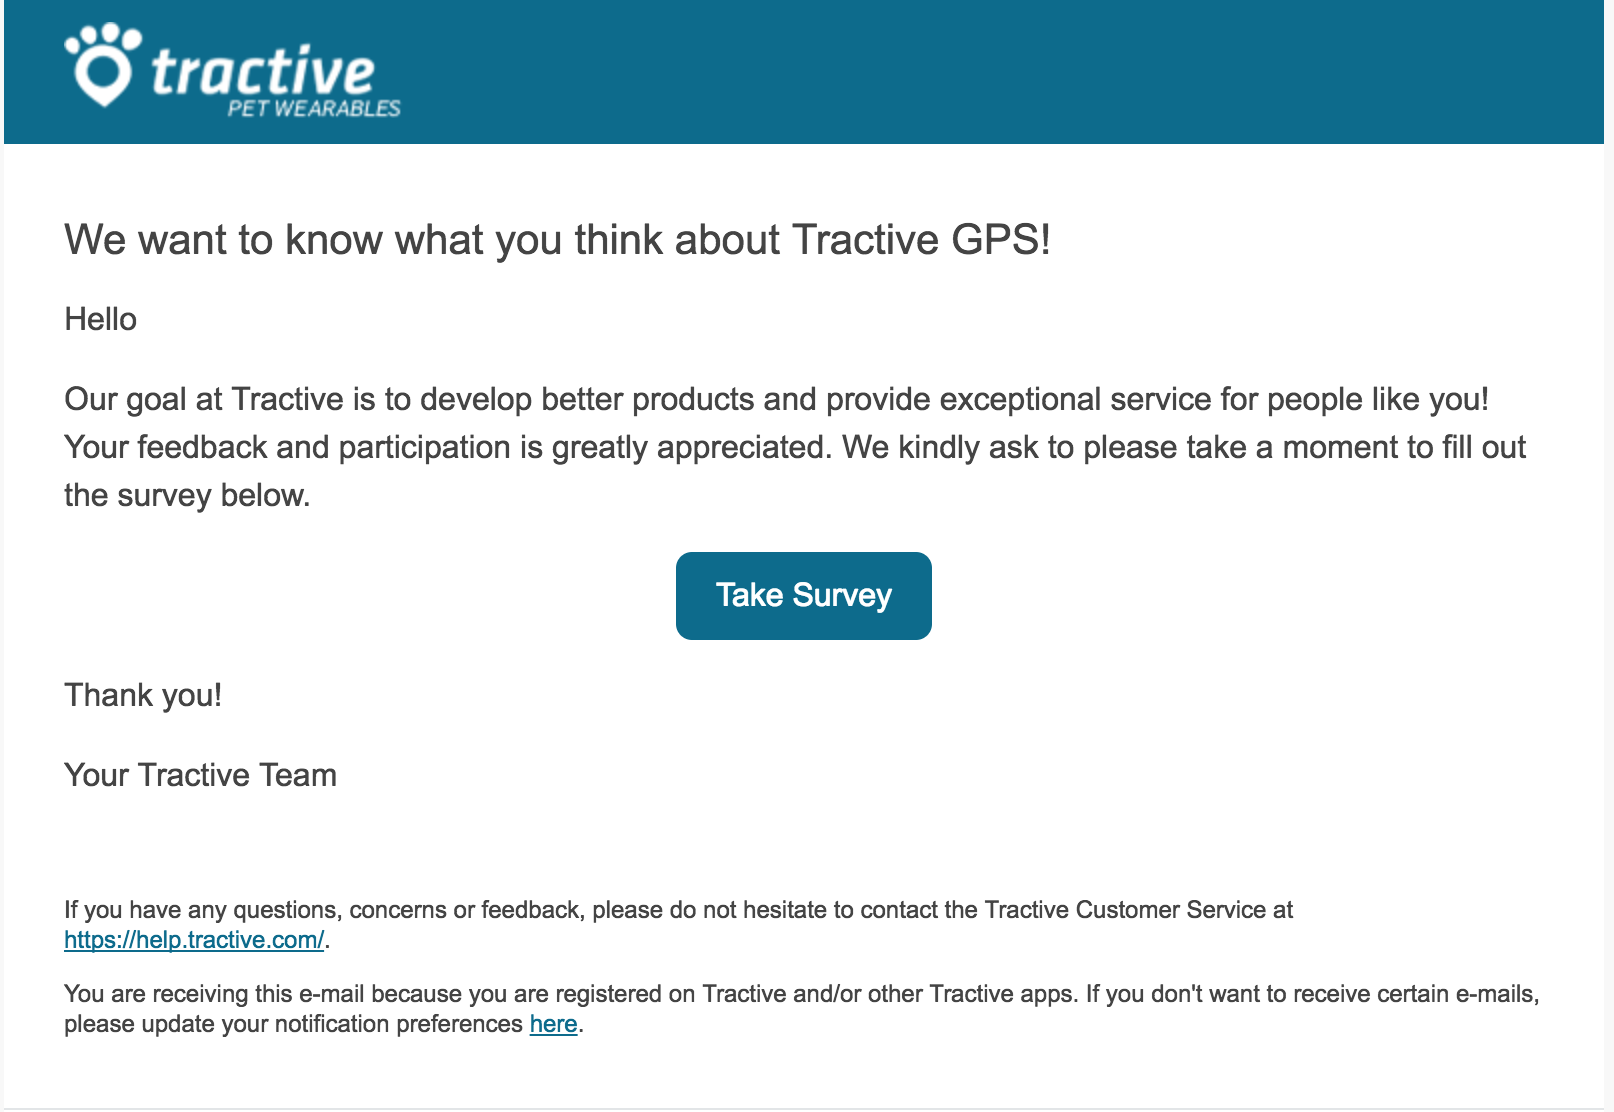
\includegraphics[width=0.8\textwidth]{img/customerSurveyEmail.png}
 	\caption{Customer Survey - Email}
 	\label{fig:customerSurveyEmail}
\end{figure} 

When the user clicks on the "Take Survey" button in the email, a browser window will open with the customer survey landing page. Behind the scenes In the URL (Uniform Resource Locator), the language version of the survey as well as the name of the customer is passed. For better personalization of the voluntary additional questions the name of the pet associated with the GPS device is sent as URL parameter. A necessary information is the unique id of the device since it allows to query all of the identified hardware- and position related data identified in section \ref{sec:dataSources}. For designing the customer survey the external tool Typeform was used. The following section describes briefly how the data gets extracted and integrated back into the internal database to be processable. Furthermore a few statistical details will be pointed out to get an impression with regard to the pending satisfaction analysis and prediction task.

\subsection{Results and interpretation of survey results}
To fetch the survey results from Typeform, a nightly job was implemented which uses the provided API of Typeform and gets the results from the previous day. The essential metrics from the two duty questions are extracted and along with the user- , pet- and tracker data stored in a new collection in the main database of Tractive. A typical structure of a document in this collection is illustrated in table \ref{tab:surveyResponse}.

\begin{table}[]
	\centering
	\resizebox{\columnwidth}{!}{%
	\begin{tabular}{|l|l|l|}
		\hline
		\multicolumn{1}{|c|}{\textbf{Attribute}} & \multicolumn{1}{c|}{\textbf{Datatype}} & \multicolumn{1}{c|}{\textbf{Description}} \\ \hline
		\_id & ObjectId & Unique identifier of document \\ \hline
		survey\_id & String & Typeform identifier for the particular language version \\ \hline
		submit\_date & DateTime & Date and time when customer submitted survey \\ \hline
		user\_id & ObjectId & Reference to the user \\ \hline
		tracker\_id & ObjectId & Reference to the tracker \\ \hline
		rating & Integer & Overall satisfaction (scale: 1-5) \\ \hline
		recommendation\_score & Integer & Recommendation potential (scale: 0-10) \\ \hline
	\end{tabular}%
	}
	\caption{Structure of a survey response represented in the company database}
	\label{tab:surveyResponse}
\end{table}

The rating and recommendation score are the two interesting numbers when it comes to predicting satisfaction for an arbitrary user afterwards. The customer survey was deployed to the productive environment on 03.07.2017 which yielded the first survey result submitted on 17.07.2017. As of 28.10.2017 17:42 UTC+2 following statistics regarding the survey could be extracted.

\begin{itemize}
	\item Number of customer survey emails sent: 15695
	\item Number of customers who filled in the survey: 2182
	\item Percentage of users who filled in the survey: 13.9\%
\end{itemize}

As these numbers show, the response rate of the customer survey fortunately is quite good. The collected amount of customer survey data so far should be sufficient for finding potential patterns in the data. In order to get a better understanding some descriptive statistic values for the satisfaction rating and the value indicating willigness of a customer to recommend Tractive were calculated. The results are shown in table \ref{tab:statisticDescriptive}. 

\begin{table}[]
	\centering
	\resizebox{\columnwidth}{!}{%
	\begin{tabular}{|c|c|c|c|c|c|c|c|c|}
		\hline
		\textbf{Survey metric} & \textbf{Min.} & \textbf{1. Quartile} & \multicolumn{1}{l|}{\textbf{Median}} & \multicolumn{1}{l|}{\textbf{Mean}} & \multicolumn{1}{l|}{\textbf{3. Quartile}} & \multicolumn{1}{l|}{\textbf{Max.}} & \multicolumn{1}{l|}{\textbf{Variance}} & \multicolumn{1}{l|}{\textbf{Standard dev.}} \\ \hline
		Satisfaction & 1 & 3 & 4 & 3.688 & 5 & 5 & 1.327 & 1.152 \\ \hline
		Recommendation & 0 & 6 & 8 & 7.137 & 9 & 10 & 7.574 & 2.752 \\ \hline
	\end{tabular} %
	}
	\caption{Statistical summary - Overall satisfaction and recommendation score}
	\label{tab:statisticDescriptive}
\end{table}

Based on the results it can be followed that the average customer rates his or her satisfaction with the Tractive GPS product as mostly satisfied represented by a value close to 4. Similar is the recommendation likeliness value where the average lies between 7 and 8. Since the first quartile with a value of 6 is rather high, it can be followed that 75\% of the customers are more likely to recommend Tractive to a friend or colleague. To close this statistical analysis of survey responses it can be stated that the majority of customers tend to be satisfied which had to be considered accordingly in the prediction framework outlined in more detail in the following section \ref{sec:predictionFramework}.

\subsection{Software architecture of prediction framework}
\label{sec:predictionFramework}

% TODO




 

